\section{System Architecture and Execution}
\label{sec:system}

\textsc{StratQ} is implemented as an embeddable analytical query engine over DuckDB~\cite{raasveldt2019duckdb} and Apache Arrow~\cite{apachearrow}.
Figure~\ref{fig:arch} illustrates the four-stage execution pipeline, separating one-time relational snapshot profiling from iterative, reference-model-driven evidence collection.

\begin{figure*}[t]
\centering
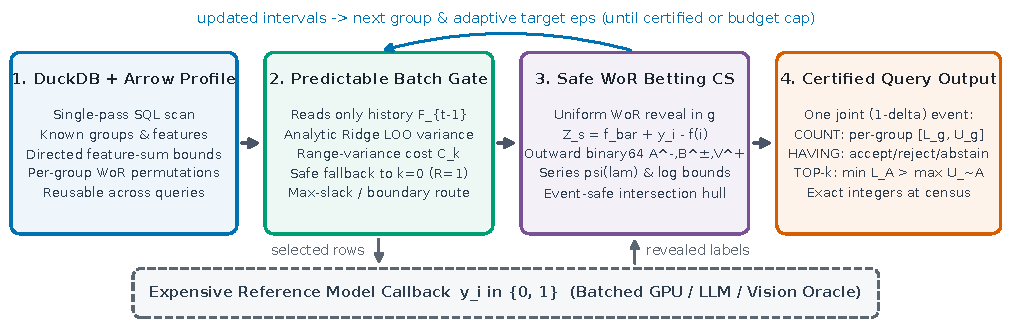
\includegraphics[width=\textwidth]{fig1_architecture.pdf}
\Description{Four-stage architecture diagram of StratQ showing DuckDB and Arrow profiling, the predictable Safe-LOO batch gate, the outward-rounded without-replacement betting confidence sequence, certified query outputs, and the batched expensive reference-model callback loop.}
\caption{\textsc{StratQ} execution architecture. One DuckDB/Arrow profiling stage materializes group indices, directed feature-sum bounds, and per-group permutations that can be reused across multiple queries. During execution, a predictable batch gate reads only revealed history $\mathcal{F}_{t-1}$, routes batched calls to the expensive reference model, and updates outward-rounded binary64 confidence sequences governing \texttt{COUNT}, \texttt{HAVING}, and \texttt{TOP-$k$} outputs.}
\label{fig:arch}
\end{figure*}

\subsection{Columnar Profiling and Arrow Transfer}
\label{sec:sys-profile}

When initialized on a Parquet file or Arrow table, \textsc{StratQ} runs one profiling stage with column pruning: only the grouping key, proxy score column, optional relational covariates, and (for offline replay) label column are projected. The stage first issues a DuckDB aggregate query for group cardinalities and feature extrema, then a column-pruned Arrow query. DuckDB exposes Arrow buffers without an obligatory copy at that boundary; conversion to Python group lists, NumPy arrays, and the stacked feature matrix materializes new arrays.
From these arrays, the profiler builds an in-memory reusable \texttt{TableProfile} containing:
\begin{enumerate}
  \item Contiguous per-group row-index slices $\{I_g\}_{g \in \mathcal{G}}$ constructed in $O(N \log N)$ via a single stable \texttt{argsort} and \texttt{bincount} split;
  \item Normalized feature matrix $\Phi \in [0, 1]^{N \times d}$ (intercept, normalized proxy score, and optional covariates);
  \item Per-group directed feature-sum envelopes $[\Phi_{\text{sum},g}^-, \Phi_{\text{sum},g}^+]$ (computed via the Higham reduction bound of \S\ref{sec:fp64}) and feature-wise extrema $[\phi_{\min,g}, \phi_{\max,g}]$.
\end{enumerate}

Crucially, for any linear predictor $f_s(i) = \theta^\top \phi_i$, the remaining-population mean $\bar{f}_s$ is updated in $O(d)$ time per revealed row by subtracting the running observed feature sum from the directed total sum interval $[\Phi_{\text{sum},g}^-, \Phi_{\text{sum},g}^+]$ and dividing by $m_s = N_g - s + 1$.
For group sizes $N_g \le 25{,}000$, \textsc{StratQ} evaluates exact linear predictor extrema $\min_{i \in I_g} \theta^\top \phi_i$ and $\max_{i \in I_g} \theta^\top \phi_i$ with outward rounding; for larger groups (e.g., 10M-row snapshots), it computes $O(d)$ outward-rounded box bounds from $[\phi_{\min,g}, \phi_{\max,g}]$, keeping per-batch metadata cost independent of $N_g$.
Because the live-callback profile stores no reference labels, its feature/group metadata can be reused across follow-up queries with different reference predicates, tolerances, thresholds $\tau_{\text{cnt}}$, or $k$ values (\S\ref{sec:eval-systems}). Offline replay instead stores the label column in the profile and is reported separately; in both modes the predictor features are specific to the profiled proxy/covariates.

\subsection{Unified Execution Loop and Adaptive Routing}
\label{sec:sys-exec}

Algorithm~\ref{alg:stratq} unifies execution across \texttt{COUNT}, \texttt{HAVING}, and \texttt{TOP-$k$}.
At query start, the engine draws an independent uniform permutation $\pi_g$ per group (never exposed to the predictor or scheduler beyond revealed prefixes) and reveals a small uniform pilot prefix $p_0$ per group, capped by $N_g$ and $B_{\max}$.
Input validation strictly enforces $y_i \in \{0, 1\}$ (rejecting \texttt{NaN} or out-of-domain outputs) and verifies that the reference callback returns exactly one label per requested row ID.

\begin{algorithm}[t]
\small
\caption{\textsc{StratQ} Certified Grouped Query Execution}
\label{alg:stratq}
\KwIn{Profile $\mathcal{P}$, reference callback $\mathcal{O}$, query mode $Q \in \{\texttt{COUNT}, \texttt{HAVING}, \texttt{TOP-}k\}$, risk $\delta$, batch size $b$, pilot $p_0$, budget cap $B_{\max}$}
\KwOut{Certified intervals $\{[L_g, U_g]\}_{g\in\mathcal{G}}$ and query-specific decision}
Initialize per-group risk $\alpha_g \leftarrow \delta/G$, uniform permutation $\pi_g$, and safe CS state $\mathcal{C}_g$ from $\mathcal{P}$\;
Reveal pilot prefix of $\min(p_0, N_g)$ rows per group under the fixed raw-proxy initialization $\theta_{\text{init}}=(0,1,0,\ldots)$ (respecting $B_{\max}$)\;
$t_{\text{total}} \leftarrow \sum_g t_g$\;
\While{$t_{\text{total}} < B_{\max}$ \textbf{and} not \textsc{Certified}$(Q, \{\mathcal{C}_g\})$}{
  Periodically refit pooled ridge $\theta_{\text{global}}$ on all revealed labels $\mathcal{F}_{t-1}$\;
  Select next group(s) $\mathcal{S} \leftarrow \textsc{Route}(Q, \{\mathcal{C}_g\})$ using only $\mathcal{F}_{t-1}$\;
  \lIf{$\mathcal{S} = \emptyset$}{\textbf{break}}
  \ForEach{$g \in \mathcal{S}$}{
    Compute predictable target $\epsilon_{\text{eff}}$ from $Q$ and $\mathcal{C}_g$\;
    $(\theta_g, [f_{\min,g}^-, f_{\max,g}^+]) \leftarrow \textsc{SafeLOOGate}(\mathcal{F}_{t-1}, g, \theta_{\text{global}}, \epsilon_{\text{eff}})$\;
    $k \leftarrow \min(b, N_g - t_g, B_{\max} - t_{\text{total}})$; \lIf{$k = 0$}{\textbf{continue}}
    $\text{rows} \leftarrow \pi_g[t_g : t_g + k]$; \quad $y \leftarrow \mathcal{O}(\text{rows})$\;
    Update $\mathcal{C}_g$ in reveal order with outward binary64 rounding; $t_g \leftarrow t_g + k$; $t_{\text{total}} \leftarrow t_{\text{total}} + k$\;
  }
}
\Return{Count intervals $\{[L_g, U_g]\}$ (exact integers at $t_g=N_g$) and certified decision / abstention for $Q$}\;
\end{algorithm}

\paragraph{Query-specific routing policies}
All three routing rules inspect only revealed interval state $\mathcal{F}_{t-1}$:
\begin{itemize}
  \item \textbf{Grouped \texttt{COUNT} (width-first max-slack).} Score each non-exhausted group by its normalized slack $s_g = \frac{(U_g - L_g)/2}{\max(\epsilon_g, 10^{-12})}$ if $(U_g - L_g)/2 > \epsilon_g$, else $0$. Route the next batch to $g^* = \arg\max_g s_g$.
  \item \textbf{Grouped \texttt{HAVING} (unresolved-boundary width-first).} Identify unresolved groups satisfying $L_g < \tau_{\text{cnt}} \le U_g$; route the next batch to the unresolved group with the largest normalized rate half-width $(U_g - L_g)/(2 N_g)$. Stop once no unresolved groups remain.
  \item \textbf{Grouped \texttt{TOP-$k$} (LUCB-style boundary pair).} Rank groups by interval midpoint (ties broken by stable secondary key) into candidate top-$k$ set $A$ and complement $\mathcal{G} \setminus A$. Let $g_{\text{in}} = \arg\min_{g \in A} L_g$ and $g_{\text{out}} = \arg\max_{h \notin A} U_h$. If $L_{g_{\text{in}}} > U_{g_{\text{out}}}$, certify $A$ and stop. Otherwise, draw from the non-exhausted members of $\{g_{\text{in}}, g_{\text{out}}\}$ (falling back to the widest non-exhausted group if both boundary groups reached census while other intervals still overlap).
\end{itemize}

\paragraph{Scalar directed-rounding engineering}
During profiling of our initial \texttt{safe\_rounding=True} implementation, we observed that dispatching scalar binary64 enclosures through NumPy array checks (\texttt{np.asarray}/\texttt{np.all}) and recomputing the 96-term $\psi(\lambda)$ series inside Python loops caused 2,280 reveal steps to take 7.69\,s (and 32,512 steps at 10M rows to take 276.5\,s).
Replacing the inner scalar enclosures with native Python \texttt{float}/\texttt{math.nextafter} fast paths and LRU-caching \texttt{psi\_e\_enclosure} (preserving bit-for-bit identical outward bounds and verified against the 50-digit \texttt{Decimal} suite) reduced the same 2,280-step benchmark from 7,689.2\,ms to 209.9\,ms ($36.6\times$ speedup) and reduced 10M-row warm query time to 2.83\,s (\S\ref{sec:eval-systems}).
This makes the statistical engine overhead negligible relative to GPU neural or LLM reference inference.
